\documentclass[11pt,letterpaper]{article}
\usepackage[margin=0.75in]{geometry}
\usepackage{mathptmx,amsmath,amssymb,graphicx,booktabs,setspace,caption,url}
\usepackage[hidelinks]{hyperref}
\usepackage{float}
\hypersetup{pdftitle={When does data quality help human deferral? Governance-constrained review allocation in knowledge-based decision systems},pdfauthor={Yeshwanth Reddy Kunam},pdfsubject={Short communication},pdfkeywords={Knowledge-based systems, learning to defer, data quality, AI governance, review capacity}}
\captionsetup{font={small,stretch=2},labelfont=bf}
\setlength{\parindent}{1em}
\setlength{\parskip}{0pt}
\setlength{\textfloatsep}{8pt}
\setlength{\intextsep}{6pt}
\widowpenalty=10000
\clubpenalty=10000
\newcommand{\TableOne}{%
\begin{tabular}{lccccc}\toprule
Method & German & Australian & Default & Macro & HMEQ (natural) \\\midrule
Automation only (rules ignored)$^a$ & 0.6254 & 0.4046 & 0.6291 & 0.5530 & 0.2583 \\
Random & 0.6327 & 0.4752 & 0.6012 & 0.5697 & 0.2700 \\
Confidence & 0.6045 & \textbf{0.4139} & 0.5700 & 0.5295 & \textbf{0.1847} \\
Chow cost risk \cite{chow} & \textbf{0.5987} & 0.4204 & 0.5684 & \textbf{0.5291} & 0.2288 \\
Quality only & 0.6514 & 0.4807 & 0.5901 & 0.5741 & 0.2960 \\
Single-head gain (earlier version) & 0.6123 & 0.4329 & 0.5634 & 0.5362 & 0.2065 \\
L2D-CE \cite{mozannar} & 0.6219 & 0.4469 & 0.5695 & 0.5461 & 0.2182 \\
L2D-OvA \cite{verma} & 0.6086 & 0.4247 & \textbf{0.5604} & 0.5312 & 0.2103 \\
Differential triage \cite{raghu} & 0.6108 & 0.4352 & 0.5657 & 0.5372 & 0.2082 \\
Two-head, probability only & 0.6100 & 0.4338 & 0.5705 & 0.5381 & 0.2163 \\
Two-head, quality-aware (proposed) & 0.6104 & 0.4338 & 0.5622 & 0.5355 & 0.2053 \\
Oracle (uses labels)$^b$ & 0.4724 & 0.2904 & 0.3692 & 0.3773 & 0.0624 \\
\bottomrule\end{tabular}}
\newcommand{\TableTwo}{%
\begin{tabular}{lccc}\toprule
Condition & Automation head only & Reviewer head only & Both heads (proposed) \\\midrule
Informative missingness (B) & $+$2.83 (20)$^{\dagger}$ & $-$0.28 (7) & $+$2.29 (18)$^{\dagger}$ \\
Stale records (B) & $+$0.98 (13) & $+$0.04 (10) & $+$0.91 (14) \\
Inconsistent codes (B) & $+$0.15 (10) & $-$0.23 (7) & $-$0.08 (10) \\
Visible defects (A), quality-coupled reviewer & $+$0.07 (13) & $+$0.70 (16) & $+$0.65 (16) \\
Visible defects (A), four decoupled reviewers & $+$0.18 (11) & $-$0.24 (5) & $-$0.07 (10) \\
HMEQ, natural missingness (external) & $+$4.53 (17)$^{\dagger}$ & $+$0.95 (14) & $+$5.12 (19)$^{\dagger}$ \\
\bottomrule\end{tabular}}

\begin{document}
\doublespacing
\begin{center}
{\large\bfseries When does data quality help human deferral? Governance-constrained review allocation in knowledge-based decision systems\par}
\vspace{2pt}
Yeshwanth Reddy Kunam$^{a,*}$\\
{\small $^a$Doctor of Business Administration, Midwest University, 851 Parr Road, Wentzville, MO 63385, United States\\
$^*$Correspondence: \texttt{yeshwanthkunam05@gmail.com}}
\end{center}
\vspace{-8pt}
\noindent\textit{Short communication.}

\begin{abstract}
\vspace{-4pt}
Automated decision systems must decide which records a model may settle, where scarce human review reduces loss, and whether staff can absorb review that governance rules make compulsory. We study a knowledge-based router combining a calibrated predictor, a two-rule data-quality knowledge base, a two-head loss estimator trained on incomplete review logs, and an allocator that enforces capacity and holds mandatory cases it cannot serve. Sorting solves this allocation exactly in feasible and overloaded regimes, and in a multi-period system the backlog does not depend on how mandatory cases are prioritized. Against published learning-to-defer surrogates, differential triage and cost-aware heuristics, under matched information, rules and capacity, four credit datasets, nine data-quality conditions, five simulated reviewer models and 20 corrected repeated splits, the router was the best learning-based method but 1.2\% costlier than Chow's cost-risk rule when pooled. With about 6,000 training records it beat Chow's rule and L2D-CE on all 20 splits; with a few hundred it lost. Quality signals helped mainly when missingness was informative about outcomes, by improving estimates of automated rather than reviewer error. Under data deterioration, staffing determined backlog far more than routing did.
\end{abstract}
\vspace{-6pt}
\noindent\textbf{Keywords:} Knowledge-based systems; Learning to defer; Data quality; AI governance; Human--AI collaboration; Review capacity

\section{Introduction}
AI governance links accountability to data and system controls \cite{abraham,janssen,mikalefgov,wirtz}, yet requiring human oversight does not by itself make oversight effective \cite{green}. Managers must decide which records may be automated, where review reduces expected loss, and whether staff can meet the review demand that data-quality rules make compulsory. Rejection and learning to defer (L2D) trade model error against abstention or expert error \cite{chow,zhangreject,mozannar,verma}; rejection wrappers and uncertainty quantification rank cases by confidence \cite{mena,abdar}, which does not measure review benefit; triage estimates human and model error separately \cite{raghu}; and recent work adds workload limits \cite{alves}, sparse expert data \cite{hemmer}, quality-aware cascades \cite{farinhas} and congestion \cite{congestion}. Data-management research treats completeness and validity as measurable input properties \cite{chai,iot,mohammed}, human-in-the-loop systems depend on how human effort is deployed \cite{wuhitl,tariq}, and knowledge-based credit decision support links predictions to business actions without modeling reviewer capacity \cite{onari}. Missing from this literature is an account of what happens when quality-triggered mandatory review meets fixed capacity: records that cannot be reviewed are neither automated nor resolved, and a quality signal may predict model error, reviewer error, both or neither.

An earlier version of this study found only a 0.2\% advantage of quality-aware gain over a feature-aware comparator, using a reviewer simulated from the router's own quality signals and no published baselines. We therefore ask: \textit{under what data-quality and review-capacity conditions does quality-aware deferral reduce decision cost while satisfying explicit governance rules?} Contributions: (i) an exact solution of governance-constrained allocation in both regimes, correcting the earlier overload rule, and a proof that backlog is invariant to prioritization; (ii) a two-head estimator that learns from incomplete review logs; (iii) a matched comparison with published L2D and triage methods under reviewers that do not favor the proposed representation, defects invisible to quality checks, and an external dataset; and (iv) a conditions analysis with managerial backlog outcomes. We claim neither a new surrogate loss nor the first quality-aware router.

\section{Method}
For record $i$ in a batch of $n$, a calibrated predictor gives $p_i$; with costs $c_{FN}=5$, $c_{FP}=1$, the automated decision is $\hat y_i=\mathbf 1[p_i\ge 1/6]$ with loss $\ell^A_i=w(y_i)\mathbf 1[\hat y_i\ne y_i]$, $w(1)=5$, $w(0)=1$. A reviewer errs with probability $e_i$, giving expected loss $\ell^H_i=w(y_i)e_i$; review costs $c_R=0.05$ and an unresolved (held) record $c_H=1.5$. Observable quality $q_i=(u_i,v_i)$ is the missing-field and out-of-range fraction, with bounds $[Q_{.01,j}-0.1t_j,\,Q_{.99,j}+0.1t_j]$, $t_j=\max(Q_{.99,j}-Q_{.01,j},1)$, from predictor-training rows. The knowledge base marks record $i$ mandatory, $m_i=\mathbf 1[u_i\ge 0.5\lor v_i\ge 0.25]$; thresholds are illustrative organizational policy. With actions $a_i,r_i,h_i\in\{0,1\}$ (automate, review, hold) and capacity $B=\lfloor bn\rfloor$, the router solves
\begin{equation}
\min\tfrac1n\textstyle\sum_i\big[a_i\ell^A_i+r_i(\ell^H_i+c_R)+h_ic_H\big]
\label{eq:obj}
\end{equation}
subject to $a_i+r_i+h_i=1$, $\sum_ir_i\le B$, $a_i\le 1-m_i$, $h_i\le m_i$ and the service-first constraint $\sum_ih_i=(|M|-B)^+$, $M=\{i:m_i=1\}$. Let $g_i=\ell^A_i-\ell^H_i-c_R$.

\textbf{Proposition 1.} \textit{If $|M|\le B$, reviewing all of $M$ plus the $B-|M|$ optional records with the largest positive $g_i$ is optimal. If $|M|>B$, every feasible route reviews exactly $B$ mandatory records and no optional record; reviewing the $B$ smallest $\ell^H_i$ is optimal. Routes do not depend on $c_H$.} Proof: in the first case no record is held, so each optional review changes (\ref{eq:obj}) by $-g_i/n$ and an exchange argument applies. In the second, $B$ unheld mandatory records must be reviewed, exhausting capacity; only $\sum_{i\in R}\ell^H_i$ depends on the reviewed set $R$, and $c_H$ enters as the constant $(|M|-B)c_H$. $\square$ The earlier version ordered overloaded mandatory records by estimated gain, which wrongly includes $\ell^A_i$ for records that cannot be automated.

\textbf{Proposition 2.} \textit{When held records carry over between periods and Proposition 1 is applied each period, holds, backlog, reviews and completions in every period are identical for any ordering of mandatory records.} Proof: by induction, equal backlog implies equal $|M_t|$, hence equal holds $(|M_t|-B)^+$. $\square$ Staffing therefore sets the backlog, approximately growing by $(\mu_t-b)^+n$ per period for mandatory rate $\mu_t$, whereas prioritization only decides who waits.

Review logs are sparse in practice, so we estimate $g_i$ with two gradient-boosted regressors on the eight inputs $z_i=(p_i,\,s_i,\,q_i,\,p_iq_i,\,\hat y_iq_i)$, where $s_i=\min(5p_i,\,1-p_i)$ is the Bayes risk of automation: an \textit{automation head} $\hat\ell^A(z)$ fitted on all labelled records, and a \textit{reviewer head} $\hat\ell^H(z)$ fitted only on records with one logged review decision, using the unbiased target $w(y_i)\mathbf 1[\text{review}\ne y_i]$. Optional records are reviewed only if $\hat g_i=\hat\ell^A-\hat\ell^H-c_R>0$; overloaded mandatory records are ordered by $\hat\ell^H$. Allocation costs $O(n\log n)$, and each decision is logged as a label-free audit tuple $(p_i,q_i,m_i,\hat\ell^A_i,\hat\ell^H_i,\text{action})$, which documents routing but is not an explanation in the XAI sense \cite{arrieta,adadi,artelt}.

\section{Experimental protocol}
Credit scoring is a standard benchmark domain \cite{lessmann}. We use German (1,000 records), Australian (690) and default-of-credit-card (30,000) data \cite{german,australian,default}, and HMEQ (5,960; natural missingness in 11 of 12 predictors) as an external dataset unused during development \cite{hmeq}. Feature-identical records are grouped and split by majority label into 45\% predictor training, 15\% calibration, 20\% gain fitting and 20\% testing over seeds 2--21. A histogram gradient-boosting classifier (120 iterations, 15 leaves) is calibrated by logistic regression; loss heads are boosted regressors (100 iterations, seven leaves). Calibration and gain partitions are expanded into clean, missing, outlier and mixed copies.

Test sets face nine conditions: clean; Family A, defects visible to quality checks (missing, outliers, mixed, and a held-out severe shift with 35--75\% missing cells); and Family B, domain-valid defects never used in fitting (outcome-informative missingness, stale records whose continuous fields are deflated by 10--45\%, inconsistent but valid category codes, and a realistic mix). Five reviewer models are simulated: constant ($e=0.10$), quality-coupled ($\min(0.4,0.05+0.35u+0.25v)$, the earlier design), feature-dependent (driven by a hidden projection of clean features), AI-correlated (errors concentrated where the model errs), and adverse ($0.25$); only the second uses the router's signals. All learned methods train on noisy, incomplete logs: 40\% of gain-fitting records carry one sampled reviewer decision.

Comparators share the predictor, rules, costs and capacity: confidence ($-|p_i-1/6|$), Chow cost risk ($s_i$) \cite{chow}, quality only ($u_i+v_i$), the earlier single-head gain, L2D-CE with cost-sensitive weights \cite{mozannar}, L2D-OvA with cost-weighted examples \cite{verma} (both one-hidden-layer networks, rejector only), differential triage \cite{raghu}, and a probability-only two-head ablation. Heuristics fill capacity; learned methods review only positive deferral scores. Because splits reuse observations, intervals and $p$-values use the corrected resampled $t$-test \cite{nadeau} with Holm adjustment \cite{holm}. A 40-day simulation (100 arrivals per day, severe shift on days 11--20, held cases carried forward) measures managerial outcomes. Code, seed-level results and checksums are public (Section 6).

\section{Results and discussion}
\textbf{Comparison.} Table~\ref{tab:main} reports cost at 20\% capacity. All rule-constrained methods reviewed 19.8\% and held 6.0\% of records with zero rule violations, so differences reflect which records were reviewed. Among learning-based methods the proposed router had the lowest macro cost (0.5355), ahead of L2D-CE by 1.95\% (19 of 20 splits; corrected $p=0.014$, Holm-adjusted $p=0.11$). Chow (0.5291) and confidence (0.5295) were cheaper, and these two heuristics also had the lowest cost under each of the five reviewer models separately. The dataset columns explain why: on default data, with about 6,000 gain-fitting records, the proposed router beat Chow, confidence, L2D-CE and its probability-only ablation on all 20 splits (by 1.1--1.5\%; $p\le0.003$) and differential triage on 19, whereas on German and Australian data, with 140--200 records, it lost to Chow by 2.0\% and 3.2\%. Subsampling the default partition confirmed the dependence (Fig.~\ref{fig:volume}): the router overtook Chow at about 1,800 records, roughly 2,900 logged review decisions. The L2D surrogates, which learn a three-way decision from scratch, needed the most data.

\begin{table}[!htb]
\centering\small\renewcommand{\arraystretch}{1.55}
\caption{Expected cost per record at 20\% capacity (lower is better), averaged over eight non-clean conditions, five reviewer models and 20 splits; HMEQ is evaluated on its natural, uncorrupted data. Learned methods are trained on noisy, incomplete review logs. Bold: lowest deployable cost per column. $^a$Ignores the rules (12.6\% violations). $^b$Upper bound, not deployable.}\label{tab:main}
\TableOne
\end{table}

\begin{figure}[!htb]
\centering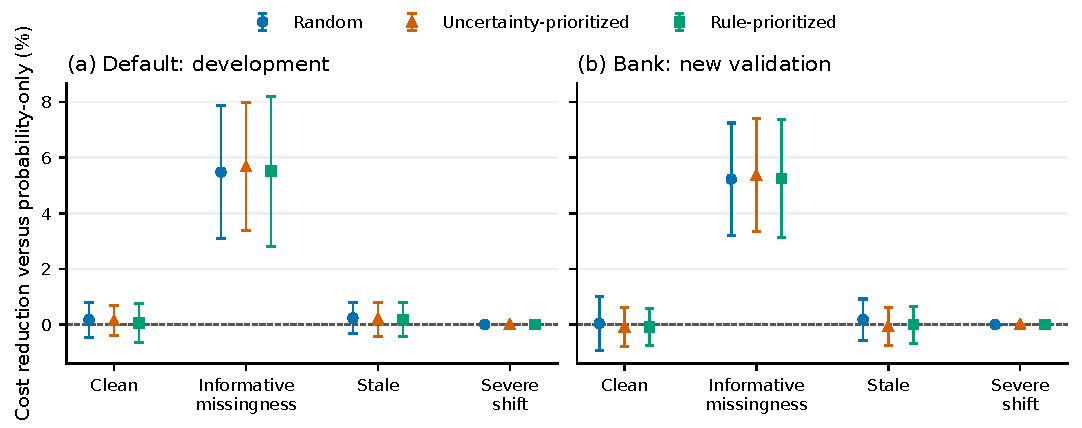
\includegraphics[width=0.84\linewidth]{budgeted_deferral/figs/fig3_volume.pdf}
\caption{Cost relative to Chow's rule as the gain-fitting partition grows (20\% capacity, 20 splits per size); negative values favor the learned router. Bands: $\pm1.96$ standard errors across splits.}\label{fig:volume}
\end{figure}

\textbf{When quality helps.} Table~\ref{tab:quality} isolates the value of quality inputs by adding them to one head at a time. Under outcome-informative missingness, quality inputs in the automation head reduced cost by 2.8\% on all 20 splits, whereas in the reviewer head they did nothing; the same pattern held on HMEQ's natural missingness ($+4.5\%$ versus $+1.0\%$). The quality signal is valuable because incompleteness predicts the model's own error. Through the reviewer head it helped only when reviewer error was constructed from quality ($+0.7\%$, 16/20, not significant), confirming that the earlier simulation favored the representation slightly. For stale records and miscoded categories, which quality checks cannot see, effects were small and unstable. Ordering overloaded mandatory records by $\hat\ell^H$ rather than by gain lowered cost by only 0.18\% ($p=0.47$), and the two-head estimator beat the single-head estimator by 0.6\% with 10--40\% of records logged but not with complete logs (both n.s.).

\begin{table}[!htb]
\centering\small\renewcommand{\arraystretch}{1.55}
\caption{Cost reduction (\%) from adding quality inputs to the two-head router relative to its probability-only version, by head, at 20\% capacity; splits won out of 20 in parentheses. Bold: corrected $p<0.05$.}\label{tab:quality}
\TableTwo
\end{table}

\textbf{Governance and managerial outcomes.} Under severe shift the rules forced 47.5\% of records into holds and raised cost by 67\% relative to an unconstrained router, which automated 54\% of policy-barred records. Stricter thresholds cut the share of truly defective records that were automated from 80\% to 4.5\% under visible shift, but left 75\% automated under invisible defects, so zero violations do not establish adequate controls. Re-optimizing every method for cost ratios of 2, 5 and 10, review fees of 0--0.2 and hold penalties of 0.5--3.0 left the ranking unchanged; hold penalties shifted cost exactly linearly with identical routes, as Proposition~1 predicts. In the 40-day simulation (Fig.~\ref{fig:backlog}), mandatory demand rose from 5.5\% to 70\% of arrivals during the episode. As Proposition~2 predicts, three prioritization rules produced identical backlogs, and the fluid estimate matched peaks of 500, 300 and 200 records at 20\%, 40\% and 50\% capacity. Raising capacity from 20\% to 40\% cut cost per arrival by 45\% and cleared all cases, whereas prioritization only redistributed waiting: first-in-first-out halved the 95th-percentile wait at 40\% capacity (13.8 to 7.1 days) but reduced two-day resolution from 65\% to 41\%. Reviewers overturned 44--49\% of reviewed decisions, which is expected under a 5:1 cost ratio and is not evidence of a poor model. For managers this implies four rules: route with a cost-aware heuristic until several thousand review outcomes are logged; staff to mandatory rather than average demand; choose the queue discipline for its service profile; and report defect coverage and unresolved-case age, not violations alone \cite{jarrahi,capability}.

\begin{figure}[!htb]
\centering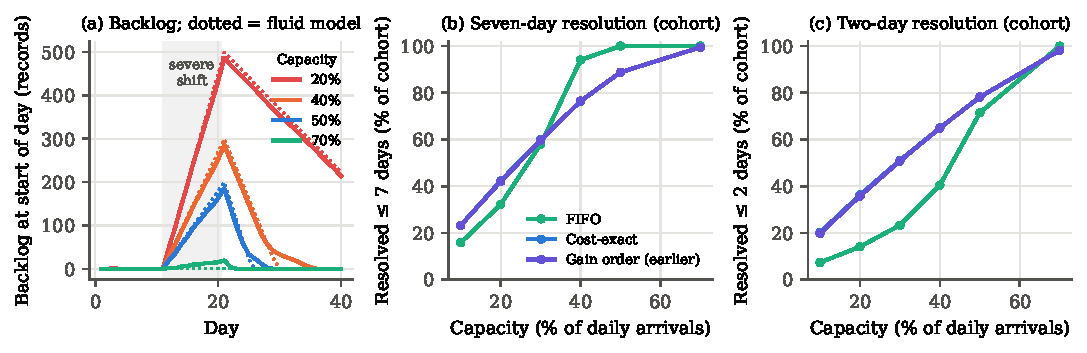
\includegraphics[width=0.97\linewidth]{budgeted_deferral/figs/fig5_backlog.pdf}
\caption{Forty-day simulation with a severe-shift episode (days 11--20). (a) Backlog at four staffing levels; dotted lines are the fluid approximation. (b) 95th-percentile wait and (c) share of mandatory cases resolved within two days, by prioritization rule (four datasets, two reviewers, ten seeds).}\label{fig:backlog}
\end{figure}

\section{Limitations}
Reviewers are simulated; real reviewers may anchor on model output, tire or change under backlog pressure, so validation with review logs is the main next step. The benchmarks are old, Family B defects are stylized, and gradual drift is not modeled \cite{lu}. Thresholds and costs are illustrative rather than elicited, although ranking was stable under refitting. Three of four prespecified hypotheses were inconclusive, the L2D baselines are adapted rather than tuned, and fairness and legal sufficiency are not assessed.

\section{Conclusion}
Exact allocation makes governance-constrained routing auditable, but its value depends on estimation. Learned routing outperformed the published deferral surrogates and, given sufficient review history, simple heuristics. Quality signals helped chiefly when missingness was informative, and under deterioration staffing, not routing, determined service completion.

\paragraph{Data and code availability}
Code, seed-level results, tables, figures and tests: \url{https://github.com/ykunam/data-quality-budgeted-deferral} (directory \texttt{budgeted\_deferral}). Datasets: \cite{german,australian,default,hmeq}. A versioned archival release (DOI) must be added before submission.

\paragraph{Declarations}
Funding, competing interests and CRediT statement: to be confirmed by the author before submission.

\paragraph{Declaration of generative AI and AI-assisted technologies in the manuscript preparation process}
ChatGPT (OpenAI) assisted with the original study design, code and drafting; Claude (Anthropic) assisted with reimplementing and extending the experiments, analysis, figures, literature checking and drafting of this revision. The author must review and verify all content and takes full responsibility for the published work.

\begingroup\small\raggedright
\begin{thebibliography}{40}
\bibitem{abraham} R. Abraham, J. Schneider, J. vom Brocke, Data governance: A conceptual framework, structured review, and research agenda, Int. J. Inf. Manag. 49 (2019) 424--438. \href{https://doi.org/10.1016/j.ijinfomgt.2019.07.008}{doi:10.1016/j.ijinfomgt.2019.07.008}.
\bibitem{janssen} M. Janssen, P. Brous, E. Estevez, L.S. Barbosa, T. Janowski, Data governance: Organizing data for trustworthy artificial intelligence, Gov. Inf. Q. 37 (2020) 101493. \href{https://doi.org/10.1016/j.giq.2020.101493}{doi:10.1016/j.giq.2020.101493}.
\bibitem{mikalefgov} E. Papagiannidis, P. Mikalef, K. Conboy, Responsible artificial intelligence governance: A review and research framework, J. Strateg. Inf. Syst. 34 (2025) 101885. \href{https://doi.org/10.1016/j.jsis.2024.101885}{doi:10.1016/j.jsis.2024.101885}.
\bibitem{wirtz} B.W. Wirtz, J.C. Weyerer, I. Kehl, Governance of artificial intelligence: A risk and guideline-based integrative framework, Gov. Inf. Q. 39 (2022) 101685. \href{https://doi.org/10.1016/j.giq.2022.101685}{doi:10.1016/j.giq.2022.101685}.
\bibitem{green} B. Green, The flaws of policies requiring human oversight of government algorithms, Comput. Law Secur. Rev. 45 (2022) 105681. \href{https://doi.org/10.1016/j.clsr.2022.105681}{doi:10.1016/j.clsr.2022.105681}.
\bibitem{chow} C. Chow, On optimum recognition error and reject tradeoff, IEEE Trans. Inf. Theory 16 (1970) 41--46. \href{https://doi.org/10.1109/TIT.1970.1054406}{doi:10.1109/TIT.1970.1054406}.
\bibitem{zhangreject} X.Y. Zhang, G.S. Xie, X. Li, T. Mei, C.L. Liu, A survey on learning to reject, Proc. IEEE 111 (2023) 185--215. \href{https://doi.org/10.1109/JPROC.2023.3238024}{doi:10.1109/JPROC.2023.3238024}.
\bibitem{mozannar} H. Mozannar, D. Sontag, Consistent estimators for learning to defer to an expert, in: Proc. 37th Int. Conf. Mach. Learn., PMLR 119 (2020) 7076--7087.
\bibitem{verma} R. Verma, E. Nalisnick, Calibrated learning to defer with one-vs-all classifiers, in: Proc. 39th Int. Conf. Mach. Learn., PMLR 162 (2022) 22184--22202.
\bibitem{mena} J. Mena, O. Pujol, J. Vitrià, Uncertainty-based rejection wrappers for black-box classifiers, IEEE Access 8 (2020) 101721--101746. \href{https://doi.org/10.1109/ACCESS.2020.2996495}{doi:10.1109/ACCESS.2020.2996495}.
\bibitem{abdar} M. Abdar, F. Pourpanah, S. Hussain, et al., A review of uncertainty quantification in deep learning: Techniques, applications and challenges, Inf. Fusion 76 (2021) 243--297. \href{https://doi.org/10.1016/j.inffus.2021.05.008}{doi:10.1016/j.inffus.2021.05.008}.
\bibitem{raghu} M. Raghu, K. Blumer, G. Corrado, J. Kleinberg, Z. Obermeyer, S. Mullainathan, The algorithmic automation problem: Prediction, triage, and human effort, arXiv preprint (2019). \url{https://doi.org/10.48550/arXiv.1903.12220}.
\bibitem{alves} J.V. Alves, D. Leitão, S. Jesus, M.O.P. Sampaio, J. Liébana, P. Saleiro, M.A.T. Figueiredo, P. Bizarro, Cost-sensitive learning to defer to multiple experts with workload constraints, Trans. Mach. Learn. Res. (2024). \url{https://openreview.net/forum?id=TAvGZm2Rqb}.
\bibitem{hemmer} P. Hemmer, L. Thede, M. Vössing, J. Jakubik, N. Kühl, Learning to defer with limited expert predictions, Proc. AAAI Conf. Artif. Intell. 37 (2023) 6002--6011. \href{https://doi.org/10.1609/aaai.v37i5.25742}{doi:10.1609/aaai.v37i5.25742}.
\bibitem{farinhas} A. Farinhas, N.M. Guerreiro, S. Agrawal, R. Rei, A. Martins, Translate smart, not hard: Cascaded translation systems with quality-aware deferral, in: Proc. 2025 Conf. Empirical Methods Nat. Lang. Process. (2025) 26742--26756. \href{https://doi.org/10.18653/v1/2025.emnlp-main.1358}{doi:10.18653/v1/2025.emnlp-main.1358}.
\bibitem{congestion} V. Saketos, W. Reveillard, A. Proutiere, S. Dalleiger, M. Xiao, To defer or not to defer? Online learning with LLMs and congested experts, arXiv preprint (2026). \url{https://doi.org/10.48550/arXiv.2610.15128}.
\bibitem{chai} C. Chai, J. Wang, Y. Luo, Z. Niu, G. Li, Data management for machine learning: A survey, IEEE Trans. Knowl. Data Eng. 35 (2023) 4646--4667. \href{https://doi.org/10.1109/TKDE.2022.3148237}{doi:10.1109/TKDE.2022.3148237}.
\bibitem{iot} L. Zhang, D. Jeong, S. Lee, Data quality management in the Internet of Things, Sensors 21 (2021) 5834. \href{https://doi.org/10.3390/s21175834}{doi:10.3390/s21175834}.
\bibitem{mohammed} S. Mohammed, L. Budach, M. Feuerpfeil, N. Ihde, A. Nathansen, N. Noack, H. Patzlaff, F. Naumann, H. Harmouch, The effects of data quality on machine learning performance on tabular data, Inf. Syst. 132 (2025) 102549. \href{https://doi.org/10.1016/j.is.2025.102549}{doi:10.1016/j.is.2025.102549}.
\bibitem{wuhitl} X. Wu, L. Xiao, Y. Sun, J. Zhang, T. Ma, L. He, A survey of human-in-the-loop for machine learning, Future Gener. Comput. Syst. 135 (2022) 364--381. \href{https://doi.org/10.1016/j.future.2022.05.014}{doi:10.1016/j.future.2022.05.014}.
\bibitem{tariq} S. Tariq, M. Baruwal Chhetri, S. Nepal, C. Paris, A$^2$C: A modular multi-stage collaborative decision framework for human--AI teams, Expert Syst. Appl. 282 (2025) 127318. \href{https://doi.org/10.1016/j.eswa.2025.127318}{doi:10.1016/j.eswa.2025.127318}.
\bibitem{onari} M.A. Onari, M.J. Rezaee, M. Saberi, M.S. Nobile, An explainable data-driven decision support framework for strategic customer development, Knowl.-Based Syst. 295 (2024) 111761. \href{https://doi.org/10.1016/j.knosys.2024.111761}{doi:10.1016/j.knosys.2024.111761}.
\bibitem{arrieta} A. Barredo Arrieta, N. Díaz-Rodríguez, J. Del Ser, et al., Explainable artificial intelligence (XAI): Concepts, taxonomies, opportunities and challenges toward responsible AI, Inf. Fusion 58 (2020) 82--115. \href{https://doi.org/10.1016/j.inffus.2019.12.012}{doi:10.1016/j.inffus.2019.12.012}.
\bibitem{adadi} A. Adadi, M. Berrada, Peeking inside the black-box: A survey on explainable artificial intelligence (XAI), IEEE Access 6 (2018) 52138--52160. \href{https://doi.org/10.1109/ACCESS.2018.2870052}{doi:10.1109/ACCESS.2018.2870052}.
\bibitem{artelt} A. Artelt, R. Visser, B. Hammer, ``I do not know! but why?'' --- Local model-agnostic example-based explanations of reject, Neurocomputing 558 (2023) 126722. \href{https://doi.org/10.1016/j.neucom.2023.126722}{doi:10.1016/j.neucom.2023.126722}.
\bibitem{lessmann} S. Lessmann, B. Baesens, H.V. Seow, L.C. Thomas, Benchmarking state-of-the-art classification algorithms for credit scoring: An update of research, Eur. J. Oper. Res. 247 (2015) 124--136. \href{https://doi.org/10.1016/j.ejor.2015.05.030}{doi:10.1016/j.ejor.2015.05.030}.
\bibitem{german} [dataset] H. Hofmann, Statlog (German Credit Data), UCI Machine Learning Repository (1994). \url{https://doi.org/10.24432/C5NC77}.
\bibitem{australian} [dataset] R. Quinlan, Statlog (Australian Credit Approval), UCI Machine Learning Repository (1987). \url{https://doi.org/10.24432/C59012}.
\bibitem{default} [dataset] I. Yeh, Default of Credit Card Clients, UCI Machine Learning Repository (2009). \url{https://doi.org/10.24432/C55S3H}.
\bibitem{hmeq} [dataset] B. Baesens, D. Rösch, H. Scheule, Credit Risk Analytics: Measurement Techniques, Applications, and Examples in SAS, Wiley, Hoboken, NJ, 2016 (HMEQ data set).
\bibitem{nadeau} C. Nadeau, Y. Bengio, Inference for the generalization error, Mach. Learn. 52 (2003) 239--281. \href{https://doi.org/10.1023/A:1024068626366}{doi:10.1023/A:1024068626366}.
\bibitem{holm} S. Holm, A simple sequentially rejective multiple test procedure, Scand. J. Stat. 6 (1979) 65--70.
\bibitem{jarrahi} M.H. Jarrahi, Artificial intelligence and the future of work: Human-AI symbiosis in organizational decision making, Bus. Horiz. 61 (2018) 577--586. \href{https://doi.org/10.1016/j.bushor.2018.03.007}{doi:10.1016/j.bushor.2018.03.007}.
\bibitem{capability} P. Mikalef, M. Gupta, Artificial intelligence capability: Conceptualization, measurement calibration, and empirical study on its impact on organizational creativity and firm performance, Inf. Manag. 58 (2021) 103434. \href{https://doi.org/10.1016/j.im.2021.103434}{doi:10.1016/j.im.2021.103434}.
\bibitem{lu} J. Lu, A. Liu, F. Dong, F. Gu, J. Gama, G. Zhang, Learning under concept drift: A review, IEEE Trans. Knowl. Data Eng. 31 (2019) 2346--2363. \href{https://doi.org/10.1109/TKDE.2018.2876857}{doi:10.1109/TKDE.2018.2876857}.
\end{thebibliography}
\endgroup
\end{document}
